\section{基于多重校验的时间隐通道构建方法设计}
\label{chap:hash:results}

本节对该时间隐通道构建方法进行总体描述,首先介绍时间隐通道的设计架构,然后展开介绍调制流程及数据转换过程,最后介绍解调过程及数据转换过程。

\subsection{设计架构}
\label{chap:hash:results:model}

\insertFigure{
	\begin{figure}
		\centering
        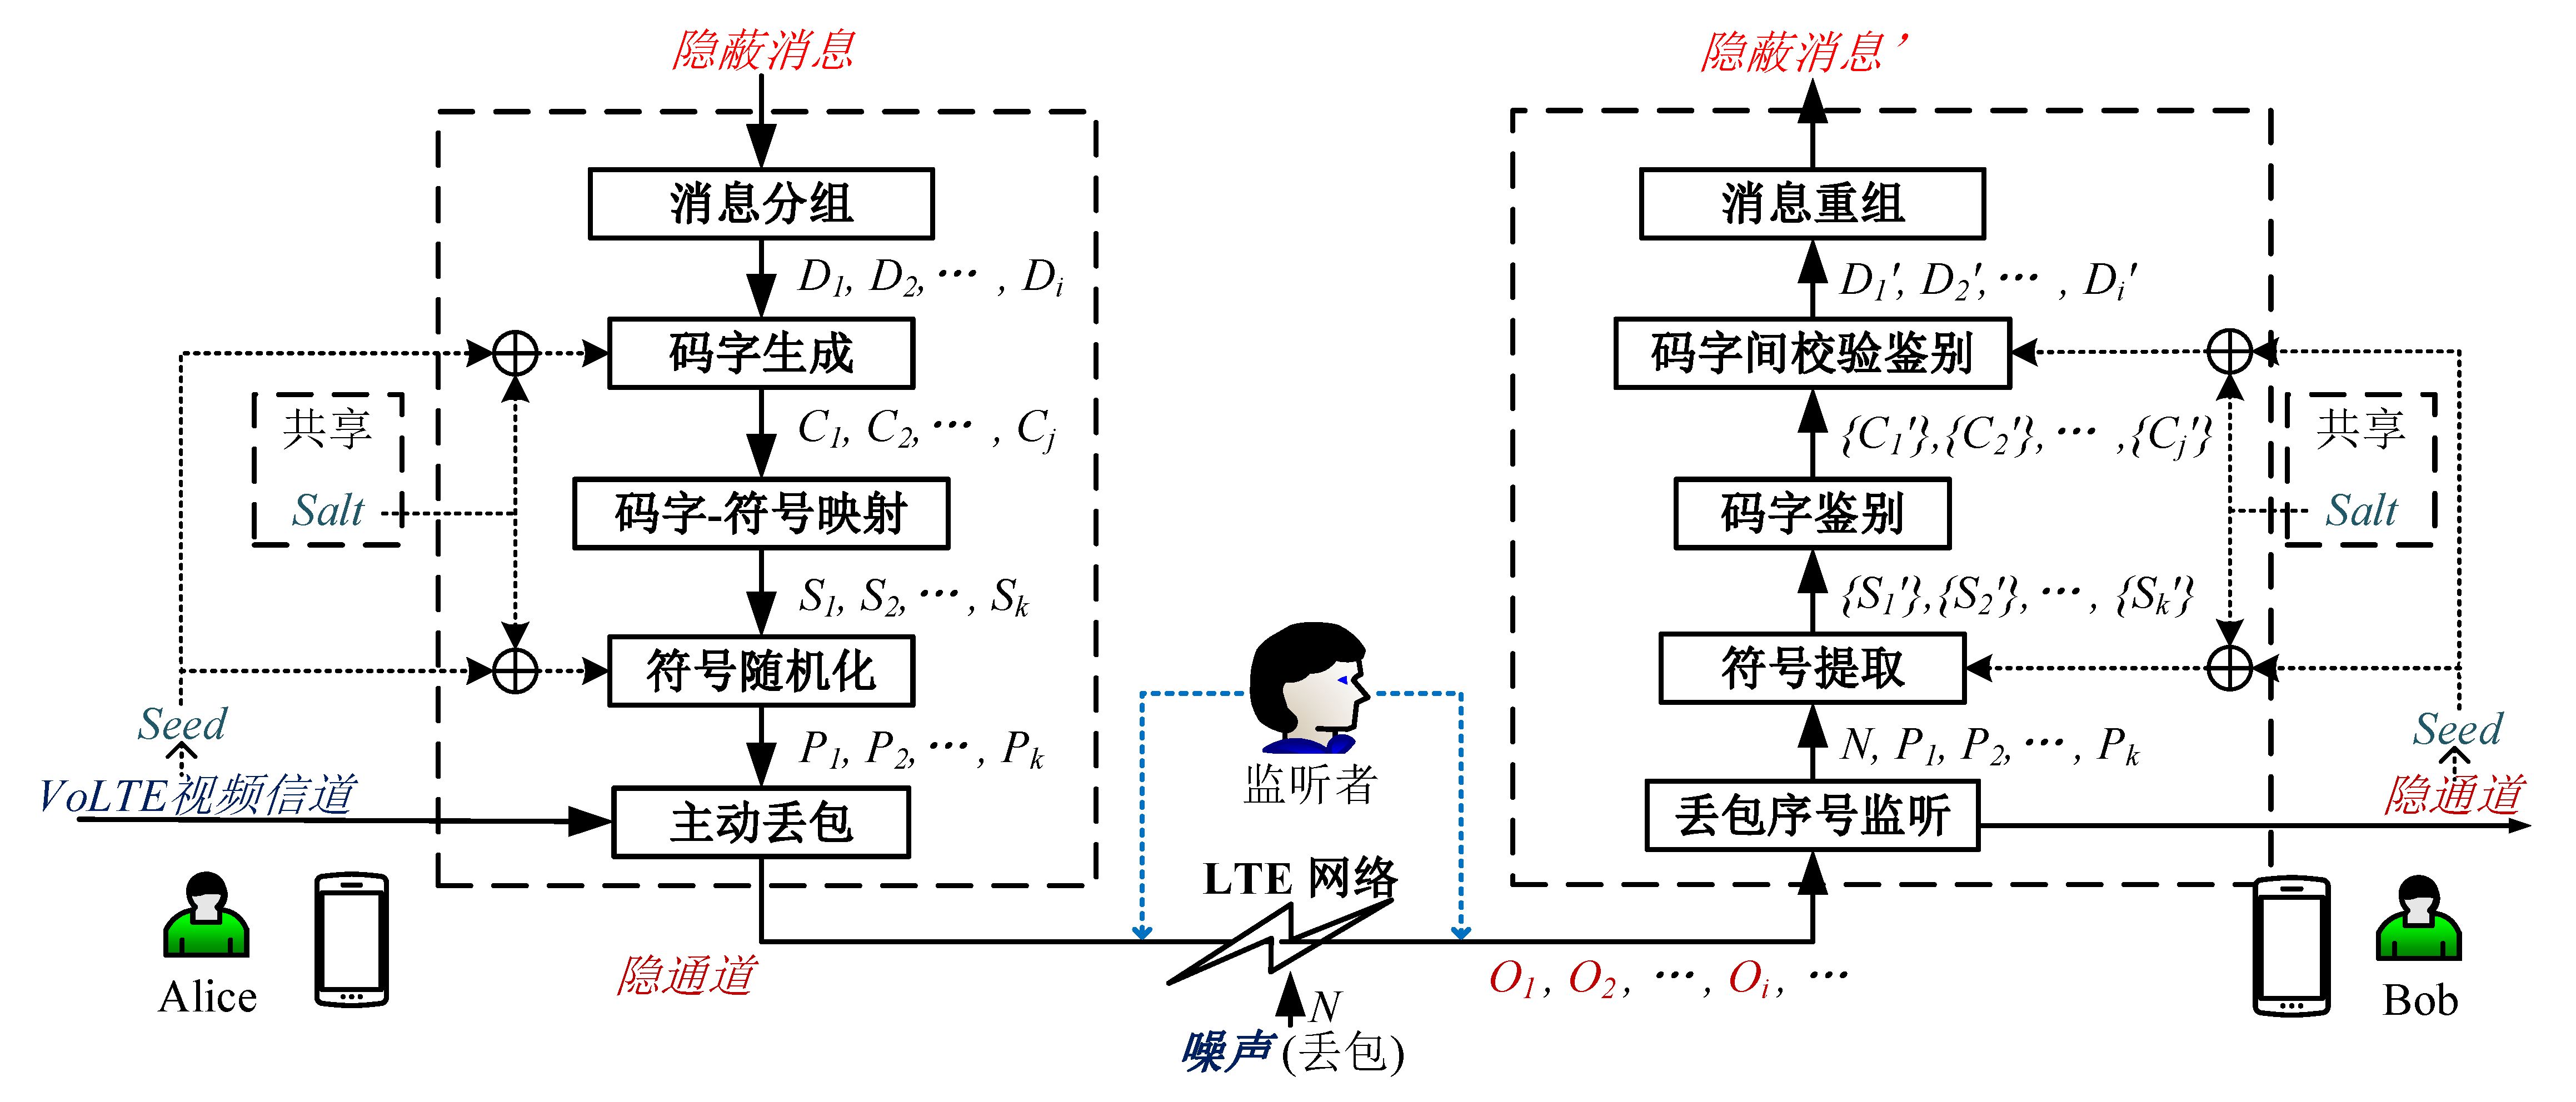
\includegraphics[width=0.99\textwidth]{chapters/chapter5/figures/system-model.pdf}
        \caption{基于多重校验的时间隐通道设计架构图}
        \label{fig:5:system-model}
    \end{figure}
}

该时间隐通道构建方法的设计架构如图\nref{fig:5:system-model},对于发送方Bob和接收方Alice来说,需要通过该时间隐通道发送隐蔽消息。为保证较保密性,双方约定一个共享的私有变量$Salt$,用于增加传输过程的随机性。发送方首先将隐蔽消息按照传输参数,进行消息分组,得到消息块$D_{i}$。接下来,码字生成过程借助私有$Salt$及RTP中的随机字段$Seed$,计算码字间校验信息及码字自校验信息,形成码字$C_{j}$。借助映射矩阵,将码字映射为符号$S_{k}$,也就是相对丢包位置。符号随机化过程对每一组的符号添加随机偏移量,并转换为要丢弃的数据包序号$P_{k}$。

宿主信道即VoLTE的视频信道,主动丢包过程将特定序号的数据包丢弃后,转变为时间隐通道,经过LTE网络传输后,到达接收方。监听者对LTE网络中的所有数据包,具有监听和控制能力。

隐通道到达接收方后,开始解调过程,通过监听数据包传输情况,得到丢失数据包序号$P_{k}$。参照映射矩阵及校验规则,符号提取过程将丢包序号转换为为候选符号集合$\{S_{k}'\}$,并验证异或校验关系。符号提取过程同时消除每组符号的随机偏移量,与调制过程添加随机偏移相同,解调过程也需要双方共享的私有$Salt$及RTP导出的$Seed$。码字鉴别过程将符号转换为候选码字,同时验证码字中基于CRC的码字自校验信息,最终输出每组的候选码字集合$\{C_{j}'\}$。码字间校验鉴别阶段,按照相同的加盐方式,对码字间的校验关系进行验证,最终筛选出概率最大的组合,并导出为消息块$D_{i}'$。最终,将消息块进行重新组合,接收方得到隐蔽消息,时间隐通道传输过程结束。

\subsection{调制流程}
\label{chap:hash:results:modulation}

\insertFigure{
    \begin{figure}
        \centering
        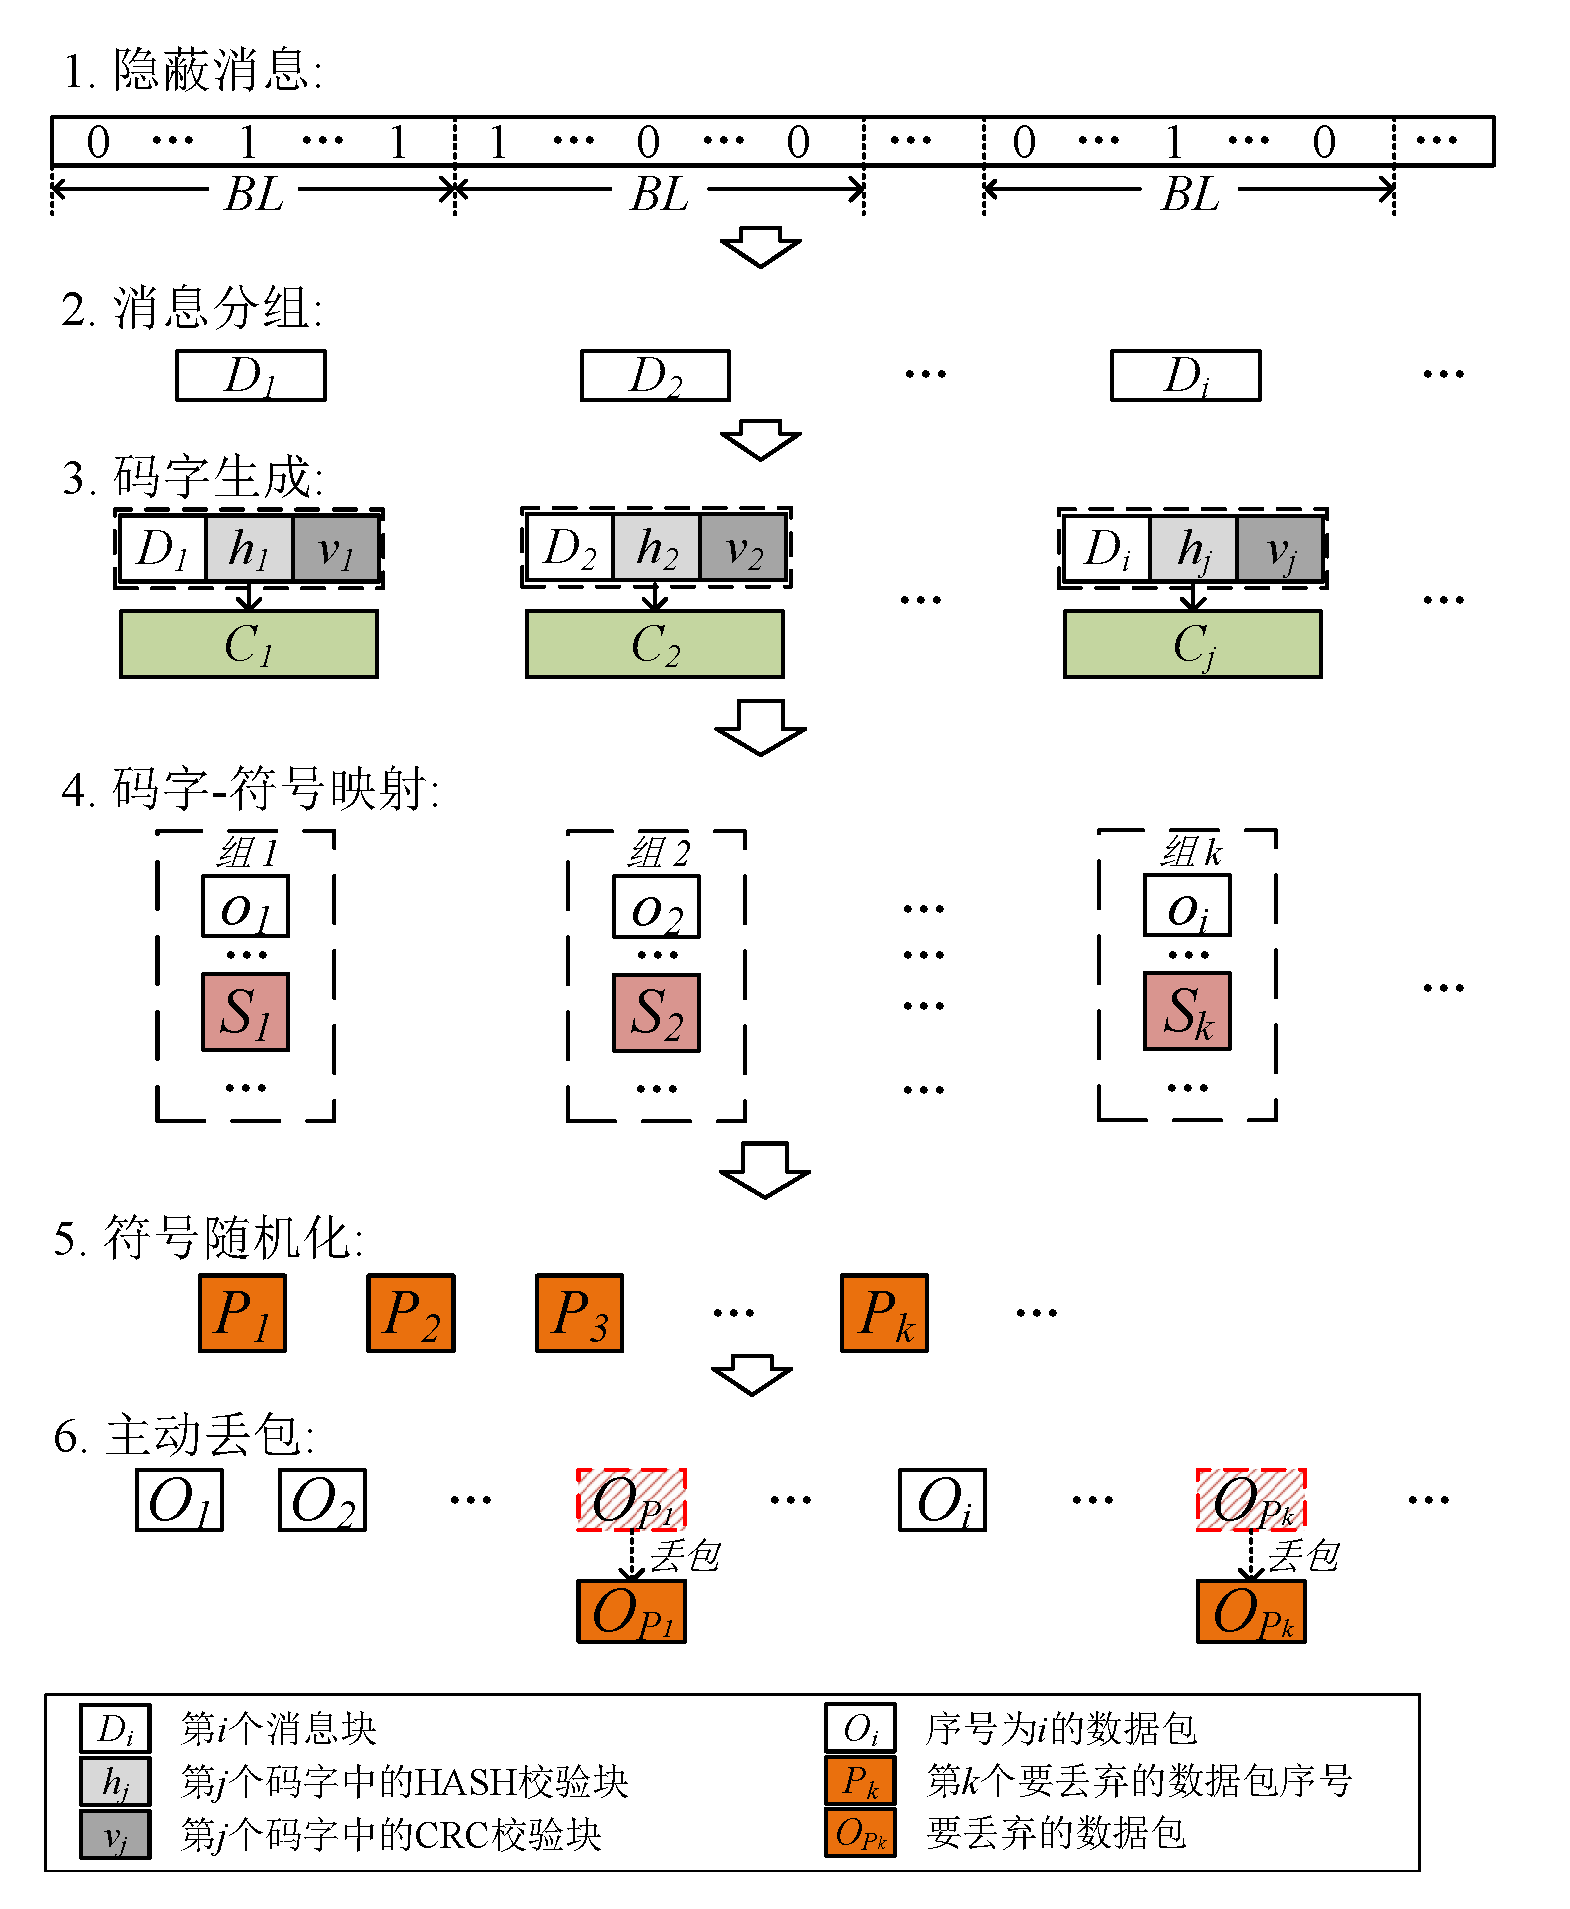
\includegraphics[width=0.85\textwidth]{chapters/chapter5/figures/modulation-flow.pdf}
        \caption{基于多重校验的时间隐通道调制流程}
        \label{fig:5:modulation-flow}
    \end{figure}

    \begin{figure}
        \centering
        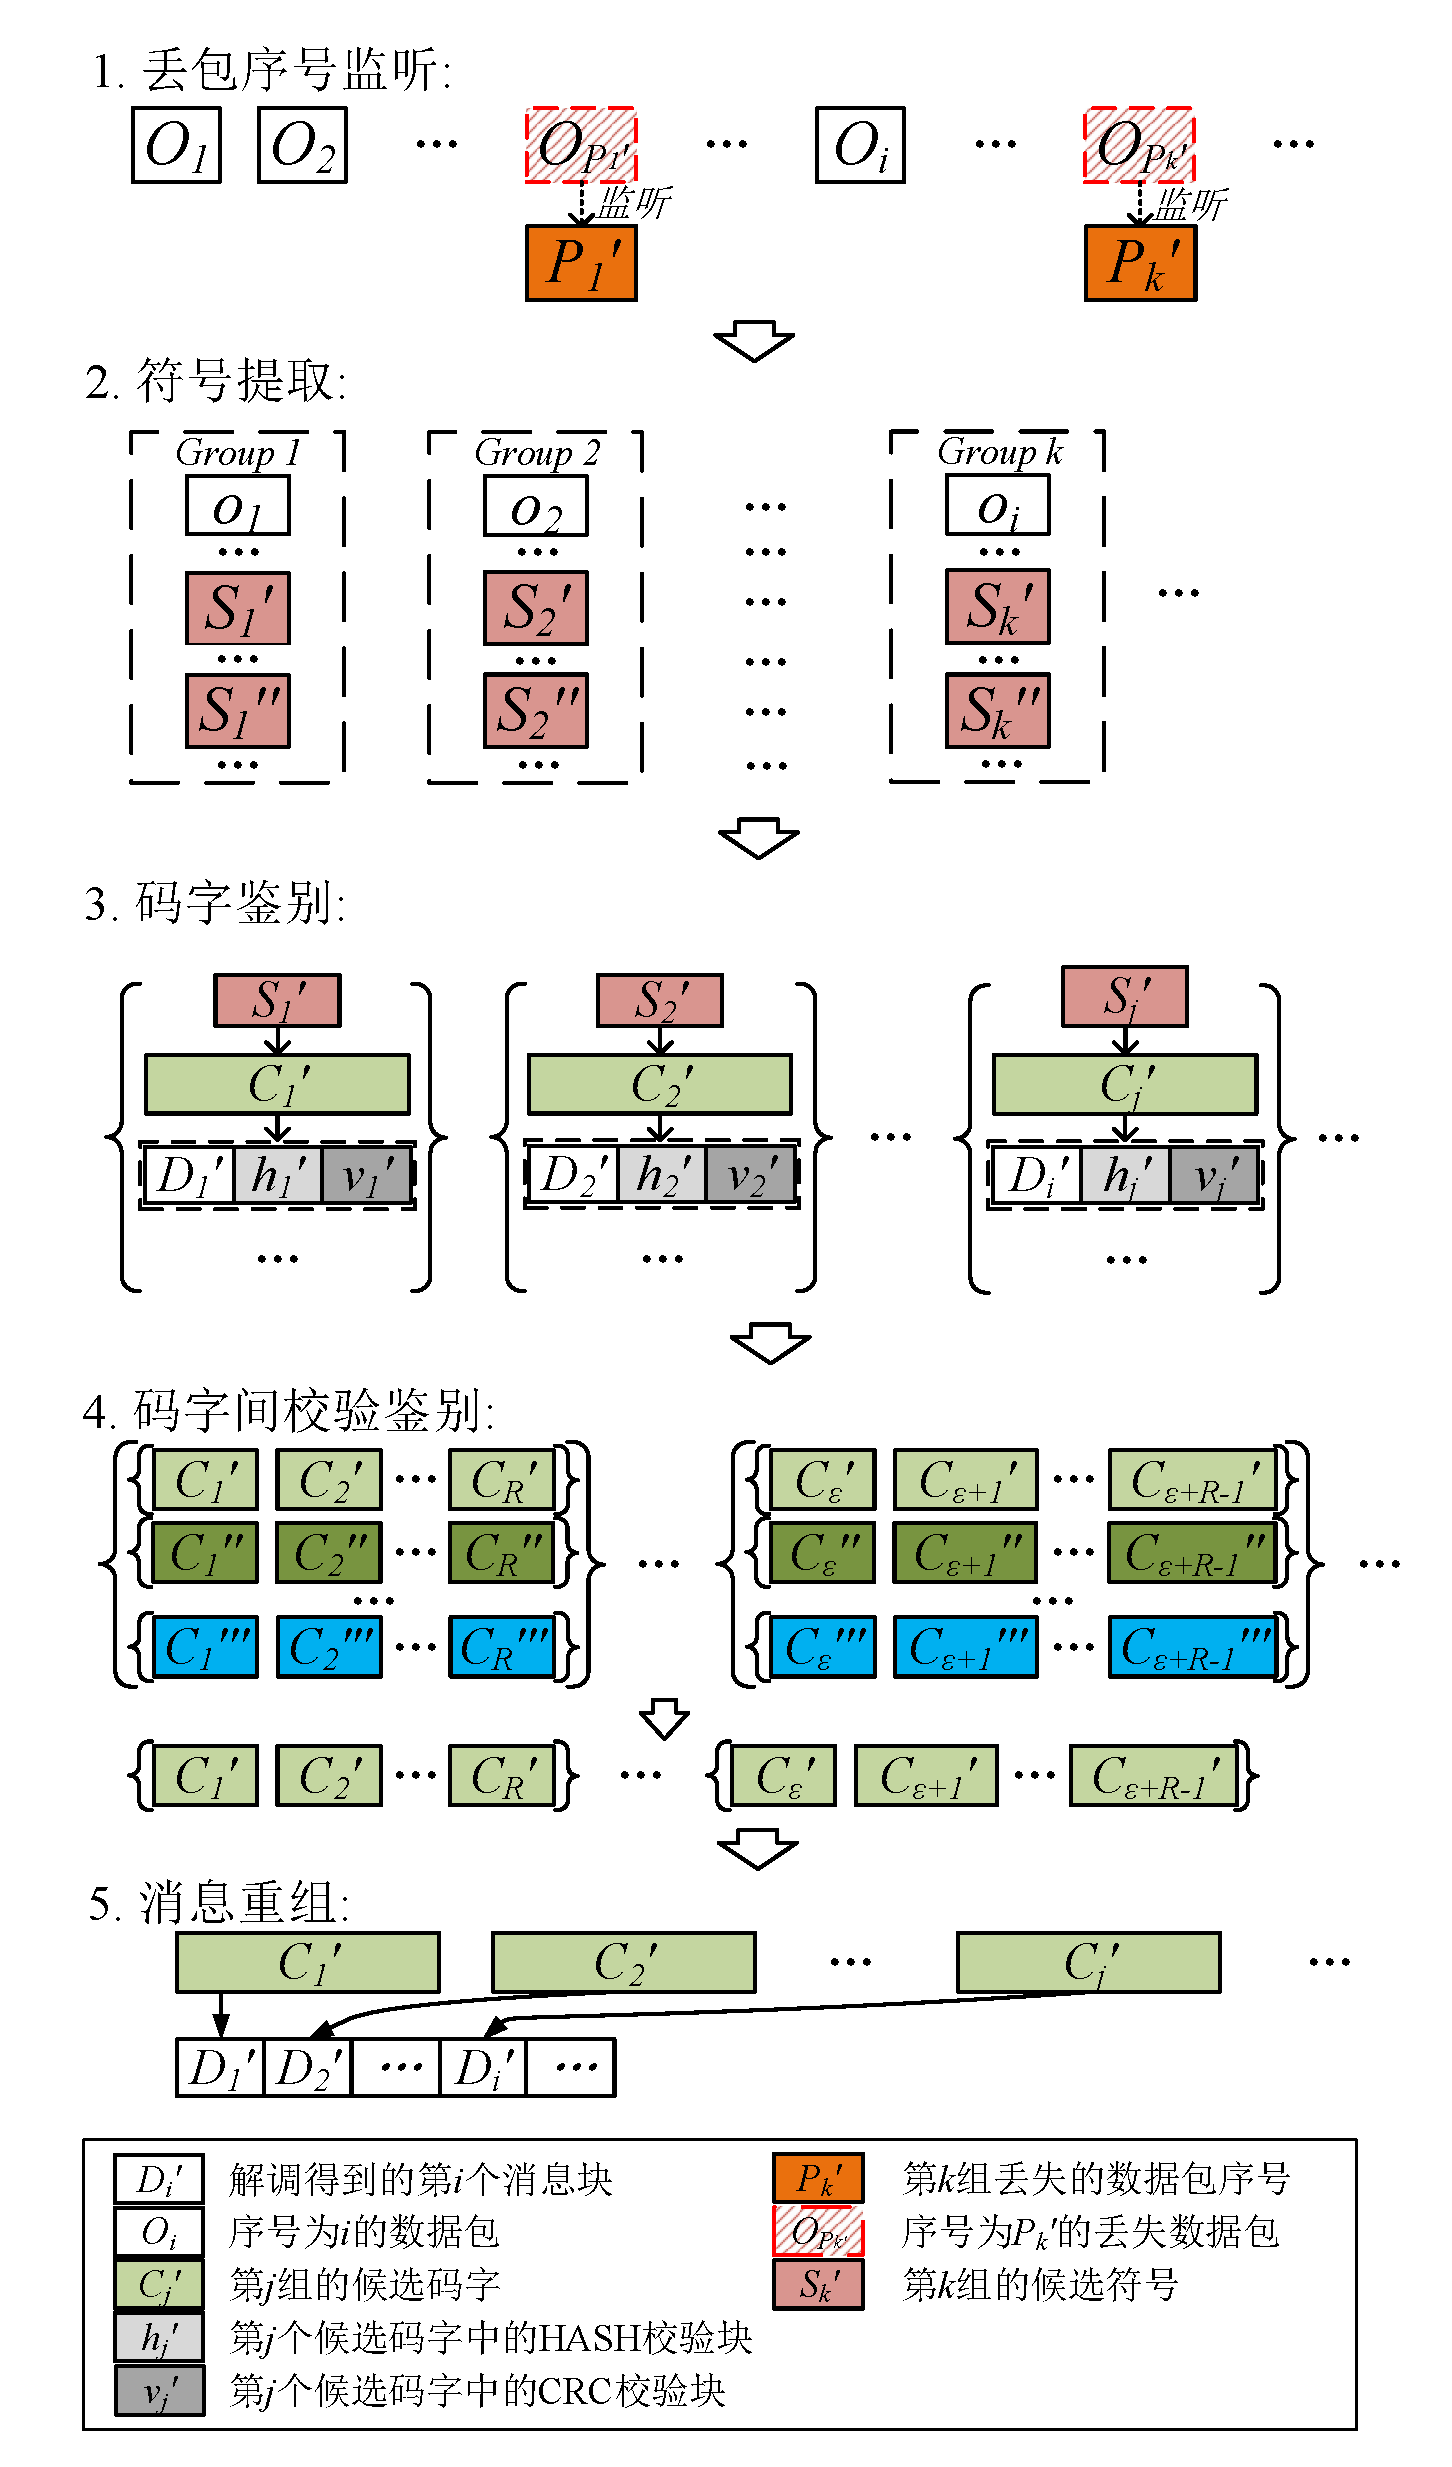
\includegraphics[width=0.75\textwidth]{chapters/chapter5/figures/demodulation-flow.pdf}
        \caption{基于多重校验的时间隐通道解调流程}
        \label{fig:5:demodulation-flow}
    \end{figure}
}

如图\nref{fig:5:modulation-flow},调制过程中的数据流变化主要分为5个部分,与时间隐通道架构中的调制流程基本一致。首先对隐蔽消息进行分组,每个数据块的长度为$BL$,得到等长数据块$\{D_{1},D_{2},\cdots , D_{i}\}$。接下来,在每个数据块的基础上,计算基于HASH的码字间校验,并将摘要结果中的$L_{HASH}$bit提取出来,作为$h_{j}$,拼接到$D_{i}$后部。对于每一个$\{D_{i}//h_{j}\}$组合,计算其CRC散列值,并将结果中的$L_{CRC}$bit作为$v_{j}$,将$\{D_{i},j_{j},v_{j}\}$按序组合,得到码字$C_{j}$。因此,$L_{Codeword}$与$BL$、$L_{HASH}$及$L_{CRC}$的关系,如公式(\nref{equ:5:codeword-length})。

\insertEquation{
    \begin{equation}
    \label{equ:5:codeword-length}
		L_{Codeword} = BL + L_{HASH} + L_{CRC}
    \end{equation}
}

码字符号映射操作,将二进制的码字$C_{j}$,转换为每组中的相对偏移量$S_{k}$。在映射矩阵中,添加额外的异或校验符号,因此最终$S_{k}$的数量要多于$C_{j}$的数量。接下来,进行符号随机化的过程,基于传入的随机数种子,迭代伪随机数发生器,为每一组符号添加随机偏移量。伪随机数发生器在保证种子一致的情况下,具有相同的随机数序列,因此保证随机数种子即可确保调制结果的随机性。通过结合用户自定义的随机数种子,及RTP中的SSRC随机字段,保证每次传输的丢包位置不同,抵御重放攻击、增强保密性。最后,将符号转换为数据包序号$P_{k}$,在主动丢包过程中,将具有序号$P_{k}$的数据包丢弃,调制过程结束。

调制过程中,影响时间隐通道抗检测能力的为参数$L_{Codeword}$,其取值决定了时间隐通道的丢包密度,通过增大$L_{Codeword}$从而获得更好的抗检测能力。影响鲁棒性的环节,包括码字生成中的参数$L_{HASH}$的$L_{CRC}$,设定更多的校验位数,即可降低码字的分布密度,噪声产生传输错误的概率降低。在保密性方面,主要由码字中的校验信息及符号中的随机偏移量两部分组成,生成$h_{j}$及$v_{j}$的源数据中均进行加盐操作,因此即使传输相同的隐蔽消息,每次生成的码字也完全不同;在随机偏移量部分,每个符号有其对应的偏移量,即使隐蔽消息不具备随机性,添加随机偏移量后具备随机特征。即使监听者获取了该时间隐通道的构建方案,并按照相同的方式进行破解,调制过程中产生的随机因素具有足够的安全保证。

\subsection{解调流程}
\label{chap:hash:results:demodulation}

如图\nref{fig:5:demodulation-flow},解调过程中的数据流程主要包括5个部分,与图\nref{fig:5:system-model}中解调过程对应。丢包序号监听分析当前接收到的数据包序号,根据序号之间的空缺情况,得到丢失数据包序号$P_{k}'$。符号提取过程将序号转变为每组的符号,在该时间隐通道中,网络噪声产生的干扰不可避免,每组中的候选符号存在不止一个的情况,因此每组的候选符号为集合$\{S_{k}',S_{k}'',\cdots \}$。

对于候选符号$\{S_{k}',S_{k}'',\cdots \}$,首先根据协商好的随机数种子,迭代伪随机数生成器,将每组符号中的随机偏移量消除,从而进行鉴别过程。在该方法的映射矩阵中,添加了对符号的异或校验,在提取符号的过程中,对异或校验关系进行验证,鉴别出符合规则的码字,进入码字鉴别过程。

码字鉴别过程,对码字中包含的$v_{j}$部分进行验证,判断符合规则的候选码字。接下来对码字中包含的$h_{j}$部分进行验证,按照码字间校验的模式,遍历所有的码字组合,出现校验失败则意味着组合无效。最终,得到一组具有最大概率的码字组合$\{C_{1}',C_{2}',\cdots, C_{j}'\}$,进入消息重组阶段。最后的消息重组过程,将码字中的数据块$D_{i}$提取出来,按照顺序组合得到隐蔽消息。

该时间隐通道构建方法,调制基础基于数据包序号,因此自身具有传输同步功能,无需同步时钟也可保证消息顺序。通过结合码字间校验、码字自校验、符号间校验及行优先映射矩阵,逐层降低噪声强度,提高时间隐通道的鲁棒性。